\chapter{Probabilistic Variational Model}
\label{chap:statistical_model}

\lettrine{G}{ranting} a system an accommodative behavior beyond a simple reaction to user input is a major and understudied challenge in \acs{hci}.
In live \acsp{hhi}, the behavior of a speaker varies also within the same behavior.
This chapter presents a statistical approach that generates variational behaviors incrementally, making it suitable for real-time use or simulation.

\pagebreak

\section{Time series representation and \aclp{gp}}
\label{sec:time_series_analysis}

The approach presented here capitalizes on the temporal aspect of spoken interaction, specifically the evolution of mutual accommodation over the course of an interaction.
This temporal aspect is addressed in the analyses done in \cref{chap:conv_analysis,chap:speech_variations_in_hhci}.
Hence, with the feature in question chronologically sampled across equal time intervals in high temporal resolution, its values can be treated as a \emph{time series}.
Time series are used for both analysis and prediction in many fields, like anomaly detection, econometrics, seismology, geophysics, and more.
Viewing accommodation as time series helps to explore it as a process evolving over time and enables a range of analysis methods.
This approach is motivated by the arguments explained in \cref{subsec:temporal_analysis}, vis.\ that representing mutual changes by merely a few points throughout an interaction or directly comparing its beginning state to its end state is not very informative and draws a rather simplistic picture (see \cref{subsec:limitations_of_did} and \cref{fig:accommodation_types} for details and examples).

Whereas the computational model introduced in \cref{chap:computational_model} grants a \ac{sds} \emph{responsiveness} per the definition in \cref{subsec:accommodation_levels}, the approach here leads to a model that grants \emph{variability}.
It can also define a \emph{profile}, e.g., by taking the mean prediction as the core behavior (see \cref{fig:gp_vacc}), but this is not the goal pursued here.
Moreover, the generative model presented in \cref{sec:clustering_and_incremental_generation} can be combined with the aforementioned computational model, e.g., to limit the degree of accommodation or to control the change rate
This variability is achieved by fitting a \emph{\ac{gp}} to each speaker.
\Acp{gp} are stochastic processes with a multivariate normal distribution for each random variable.
Therefore, a \ac{gp} provides the joint distribution for infinitely many random variables, i.e., a \emph{distribution over functions} that match the given evidence.
Specifically, \acp{gp} are used here for \emph{kriging} (\cref{subsec:interploating_data_using_kriging}), an interpolation technique used in applications in various fields, like geostatistics, economics, and astronomy, to name a few.
The utilization of \acp{gp} provides not only a continuous line with likelihoods for the observed speech productions, but also an infinite number of potential alternatives -- the variations -- that describe the speaker's vocal behavior.

\subsection{Kernel building and tuning}
\label{subsec:covariance_functions}

% \url{http://scikit-learn.org/stable/modules/gaussian_process.html}

Kernels (also called \textit{covariance functions} in the context of \acp{gp}) are a key component in \acp{gp}, as they define the statistical relationship between the input values.
In general, they define the similarity $k(x, x')$ between each pair of input points, so that $k(\cdot, \cdot)$ determines how similar the outputs $y_*$ and $y_*'$ will be. 
More formally, a covariance function can be described as $\mathcal{K}(u, v) = \phi(u) \cdot \phi(v)$, where $\phi(\cdot)$ is a function that maps the input vectors into a transformed feature space.
Which function to use is a key consideration when using \acp{gp}, as it determines the behavior of the sampled functions and the quality of the predictions it will be able to make.
Naturally, some assumptions and decisions regarding the data must be made when choosing a kernel.
A kernel's parameters are optimized to achieve functions that better fit the data, and the consistency of the resulted functions is measured using log maximum likelihood.

Since convergence analyses usually refer to the \textit{difference} between values in different production (as opposed to the values themselves), stationary kernels are more suitable for fitting \ac{gp} to them, as they are shaped by the distances between each pair of datapoint rather than their absolute values.
%That is, they fulfill $k(x_1, x_2) = k(x_1 - x_2)$.
%This list only covers a small subset of common covariance functions.
%Further kernels include the exp-sine squared, dot-product, linear, and more.
A kernel may also be composed of multiple other kernels, to capture a combination of characteristics.
This is done either by multiplication or addition of these kernels.
Multiplication-based kernels are maximized when all of its kernel factors yield high values, whereas
addition-based kernels are maximized when any of their addend kernels yield a high value.
%For example, multiplying a linear kernel by a periodic one will result in functions that are \textit{both} periodic \textit{and} with increasing amplitude as they move away from the origin.
For the modeling presented here, an additive kernel is used with constant, RBF, and noise terms (see \crefrange{eq:constant_kernel}{eq:RBF_kernel}).
The RBF term determines the general shape of the curve (see example in \cref{fig:RBF_prior_posterior}), the constant term enables shifting of the curve if necessary, and the noise term adds degrees of freedom in case the curve cannot completely fit the input signal.

The definitions of the individual kernels are as follows:

\begin{description}
	\item[Constant kernel -- ]
	is a simple kernel that assigns the same value for all input pairs.
	Since by itself it does not offer a lot of characteristic to the covariance function, it is usually used in combination with other kernels, where it scales the magnitude of the other factors, or as part of a sum kernel, in which it modifies the mean of the Gaussian process.
	It has a single parameter, the constant value, and it is defined as 
	%
	\begin{equation}
		\label{eq:constant_kernel}
		k_{constant}(C, x, x') = C\forall x_1, x_2,
	\end{equation}
	\eqname{Constant kernel}
	%
	where $C$ is the constant value parameter.
	
	\item[Noise kernel -- ]
	is a kernel used for capturing unexplained variation in the data.
	It is typically based on the constant kernel as part of a sum kernel, in which it explains the noise component of a signal.
	In this context, the constant parameter is tuned to estimate the noise level in the interlocutor's mutual change (including distortions caused by measuring and \ac{asr} errors).
	This is determined by
	%
	\begin{equation}
		\label{eq:noise_kernel}
		k_{noise}(\{noise\_level\}, x, x') =
		\begin{cases}
		C_{noise\_level}, & if\quad x_1 = x_2\\
		0, & otherwise,\\
		\end{cases}
	\end{equation}
	\eqname{Noise kernel}
	%
	where $noise\_level$ equals to the variance of the noise found in the input signal.
	
	\item[Radial-basis function (RBF) kernel --]
	also known as \emph{squared exponential kernel}, this kernel is a stationary kernel with one parameter, \emph{lengthscale} $l > 0$.
%	which can either be a scalar (isotropic variant of the kernel) or a vector with the same number of dimensions as the inputs x (anisotropic variant of the kernel).
	This kernel typically results in generally smoothed functions, with the lengthscale being associated with the long-term smoothness and degree of variability on the time dimension.
	The RBF kernel is defined as
	%
	\begin{equation}
		\label{eq:RBF_kernel}
		k_{RBF}(\{\ell\}, x, x') = \sigma^2 exp\left(\frac{\lVert x_1 - x_2 \lVert ^2_d}{2\ell^2}\right),
	\end{equation}
	\eqname{Radial basis function (squared exponential) kernel}
	%
	where $\lVert x_1 - x_2 \lVert$ is the Euclidean distance between two $d$-dimensional input points and $\sigma^2$ is a scalar factor that determines the average distance of your function away from its mean.
	\cref{fig:RBF_prior_posterior} shows prior and posterior examples of the RBF kernel.
	
%	\item[Rational quadratic kernel]
%	This kernel can be seen as a scale mixture (infinite sum) of RBF kernels with different length scales.
%	Therefore, \acp{gp} priors with this kernel expect to see functions which vary smoothly across many length scales.
%	It has two parameters: length scale $l > 0$ and scale mixture $\alpha > 0$.
%	The parameter $\alpha$ determines the relative weighting of large-scale and small-scale variations.
%	When $\alpha$ $\lim$ $\inf$, the RQ kernel is identical to the SE kernel, as described by
%	
%	\begin{equation}
%		\label{eq:RQ_kernel}
%		k_{RQ}(\{\sigma, \alpha, \ell\}, x, x') = \sigma^2 \left( 1 + \frac{\lVert x_1 - x_2 \lVert ^2}{2\alpha \ell^2} \right)^{-\alpha}.
%	\end{equation}
%	\eqname{Rational quadratic kernel}
\end{description}

\subsection{Data interpolation using kriging}
\label{subsec:interploating_data_using_kriging}
	
\begin{figure}[t]
	\centering
	\subfigure[RBF kernel prior ($length scale = 1$)]
		{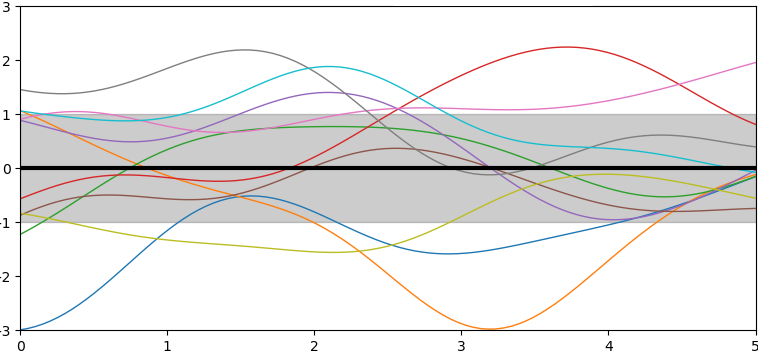
\includegraphics[width=0.45\textwidth]{RBF_prior}
	\label{fig:RBF_prior}}
	\hfill % no empty line here to avoid staring a new paragraph (figures will be vertically aligned)
	\subfigure[RBF kernel posterior ($length scale = 0.279$)]
		{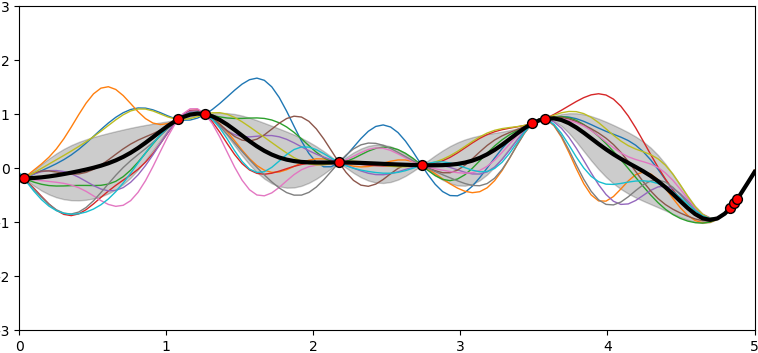
\includegraphics[width=0.45\textwidth]{RBF_posterior}
	\label{fig:RBF_posterior}}
	\caption[Prior and posterior of RBF kernel]
		{\hspace{-0.18cm}\footnotemark\ 
		Prior and posterior distributions of an RBF kernel with mean zero, resulted in a Gaussian process $\mathcal{GP}\left( 0 (\vec{x}), \Sigma(\vec{x}) \right)$.
		Each color line stands for a drawing (prediction) from the prior and posterior distributions, and the thicker black line shows the overall mean of the distributions.
		The red circles are the known datapoints on which the kernel was optimized to fit, and the gray areas mark the \SI{95}{\percent} confidence intervals above and below the overall mean.
		The length scale parameter (in parentheses) determines the length of the \enquote{wiggles} of the functions}
	\label{fig:RBF_prior_posterior}
\end{figure}
\footnotetext{adapted from \url{https://scikit-learn.org/stable/_images/sphx_glr_plot_gpr_prior_posterior_001.png}}

As also motivated in \cref{subsec:limitations_of_did,subsec:temporal_analysis}, artificially splitting interactions into a fixed, pre-determined number of parts to measure accommodation results in a partial view on the accommodation process.
To avoid that, some interpolation method is required to generate a more general behavior based on the observed productions.
This allows analysis on a continuous series of values instead of point-by-point comparison, where the temporal gaps between datapoints might be greatly unbalanced.
One way of achieving that is using \ac{loess} (see \cref{fig:hds_dds_time_pitch}), which is adequate for gaining a smooth estimation of a speaker's overall performance.
A similar approach is used in \citet{Galvez2020unifiying}, in which the average values obtained by \acl{tama} \citep[\acs{tama};][]{Kousidis2008towards, Kousidis2009monitoring} define the behavior.
However, \ac{tama} values may conceal turns with substantial changes and other tendencies that could distinguish one speaker from the other.
A more evolved approach is presented here to describe a speaker's vocal behavior in a conversation as a distribution over functions that match the accumulated \textit{evidence} from that speaker's productions.

Kriging (or \textit{\acl{gp} regression}) is an interpolation method that gives an optimally fitted and unbiased prediction of intermediate values.
Since this method fits a function distribution over the data, it not only yields mathematically more likely values, but also provides a curve that describes the characteristics of the interpolated curved, as opposed to more naive methods like linear interpolation or smoothing spline.
Another advantage of this method is that it offers a \textit{distribution over functions} rather than specific values.
Therefore, an infinite number of suitable values can be drawn from one fitted kernel and their likelihood can be evaluated.
Such interpolation is illustrated in \cref{fig:RBF_posterior}, where each line represents a mean regression prediction drawn from the posterior distribution based on the given datapoints.
To demonstrate this method, it was applied here on the dataset presented in \cref{sec:vacc}.
For simplicity, only the interactions from the solo condition were used.
The \ac{gp} prediction for each speaker can be described by
%
\begin{equation}
	\label{eq:gp_function_prediction}
	f_*(\vec{x}) = \mathcal{GP}(\mu_{\vec{x}}, \Sigma_*),
\end{equation}
\eqname{Function predicted using a fitted Gaussian process}\noindent
%
where $\mu_{conv}$ is the mean feature value of a single speaker and $\Sigma_*$ is the fitted additive covariance function described in \cref{subsec:covariance_functions}.
It is important to note that the mean is not zeroed (as usually done in \ac{gp} regression) to maintain the original input's mean for the subsequent steps.
The kernel was initialized with the priors $C = 1$, $lengthscale = 1$, and no assumptions regarding the noise level.
The search boundaries for the RBF and noise components were $1 < lengthscale < 100$ and $\num{1e-4} < \xi < 10$, respectively, with a maximum of six optimization iterations.
% the initial one plus five allowed restarts (n_restarts_optimizer parameter in code)
% \xi is here the sign for noise
The datapoints of the original series were grouped by the turn they belong to.
Then, the average values of turns immediately before and after a floor change were taken as evidence for the \ac{gp}.
This results in evidence concentrated around input from the other interlocutor, with the objective to capture turning points that are more prone to accommodation.
With the fitted kernel, a continuous prediction can be made for each speaker over the entire conversation timespan.
\Cref{fig:gp_vacc} shows an example of \ac{gp} predictions for one of the conversations.
% 20171121A_Calendar_01 was used
%
\begin{figure}[t]
	\centering
	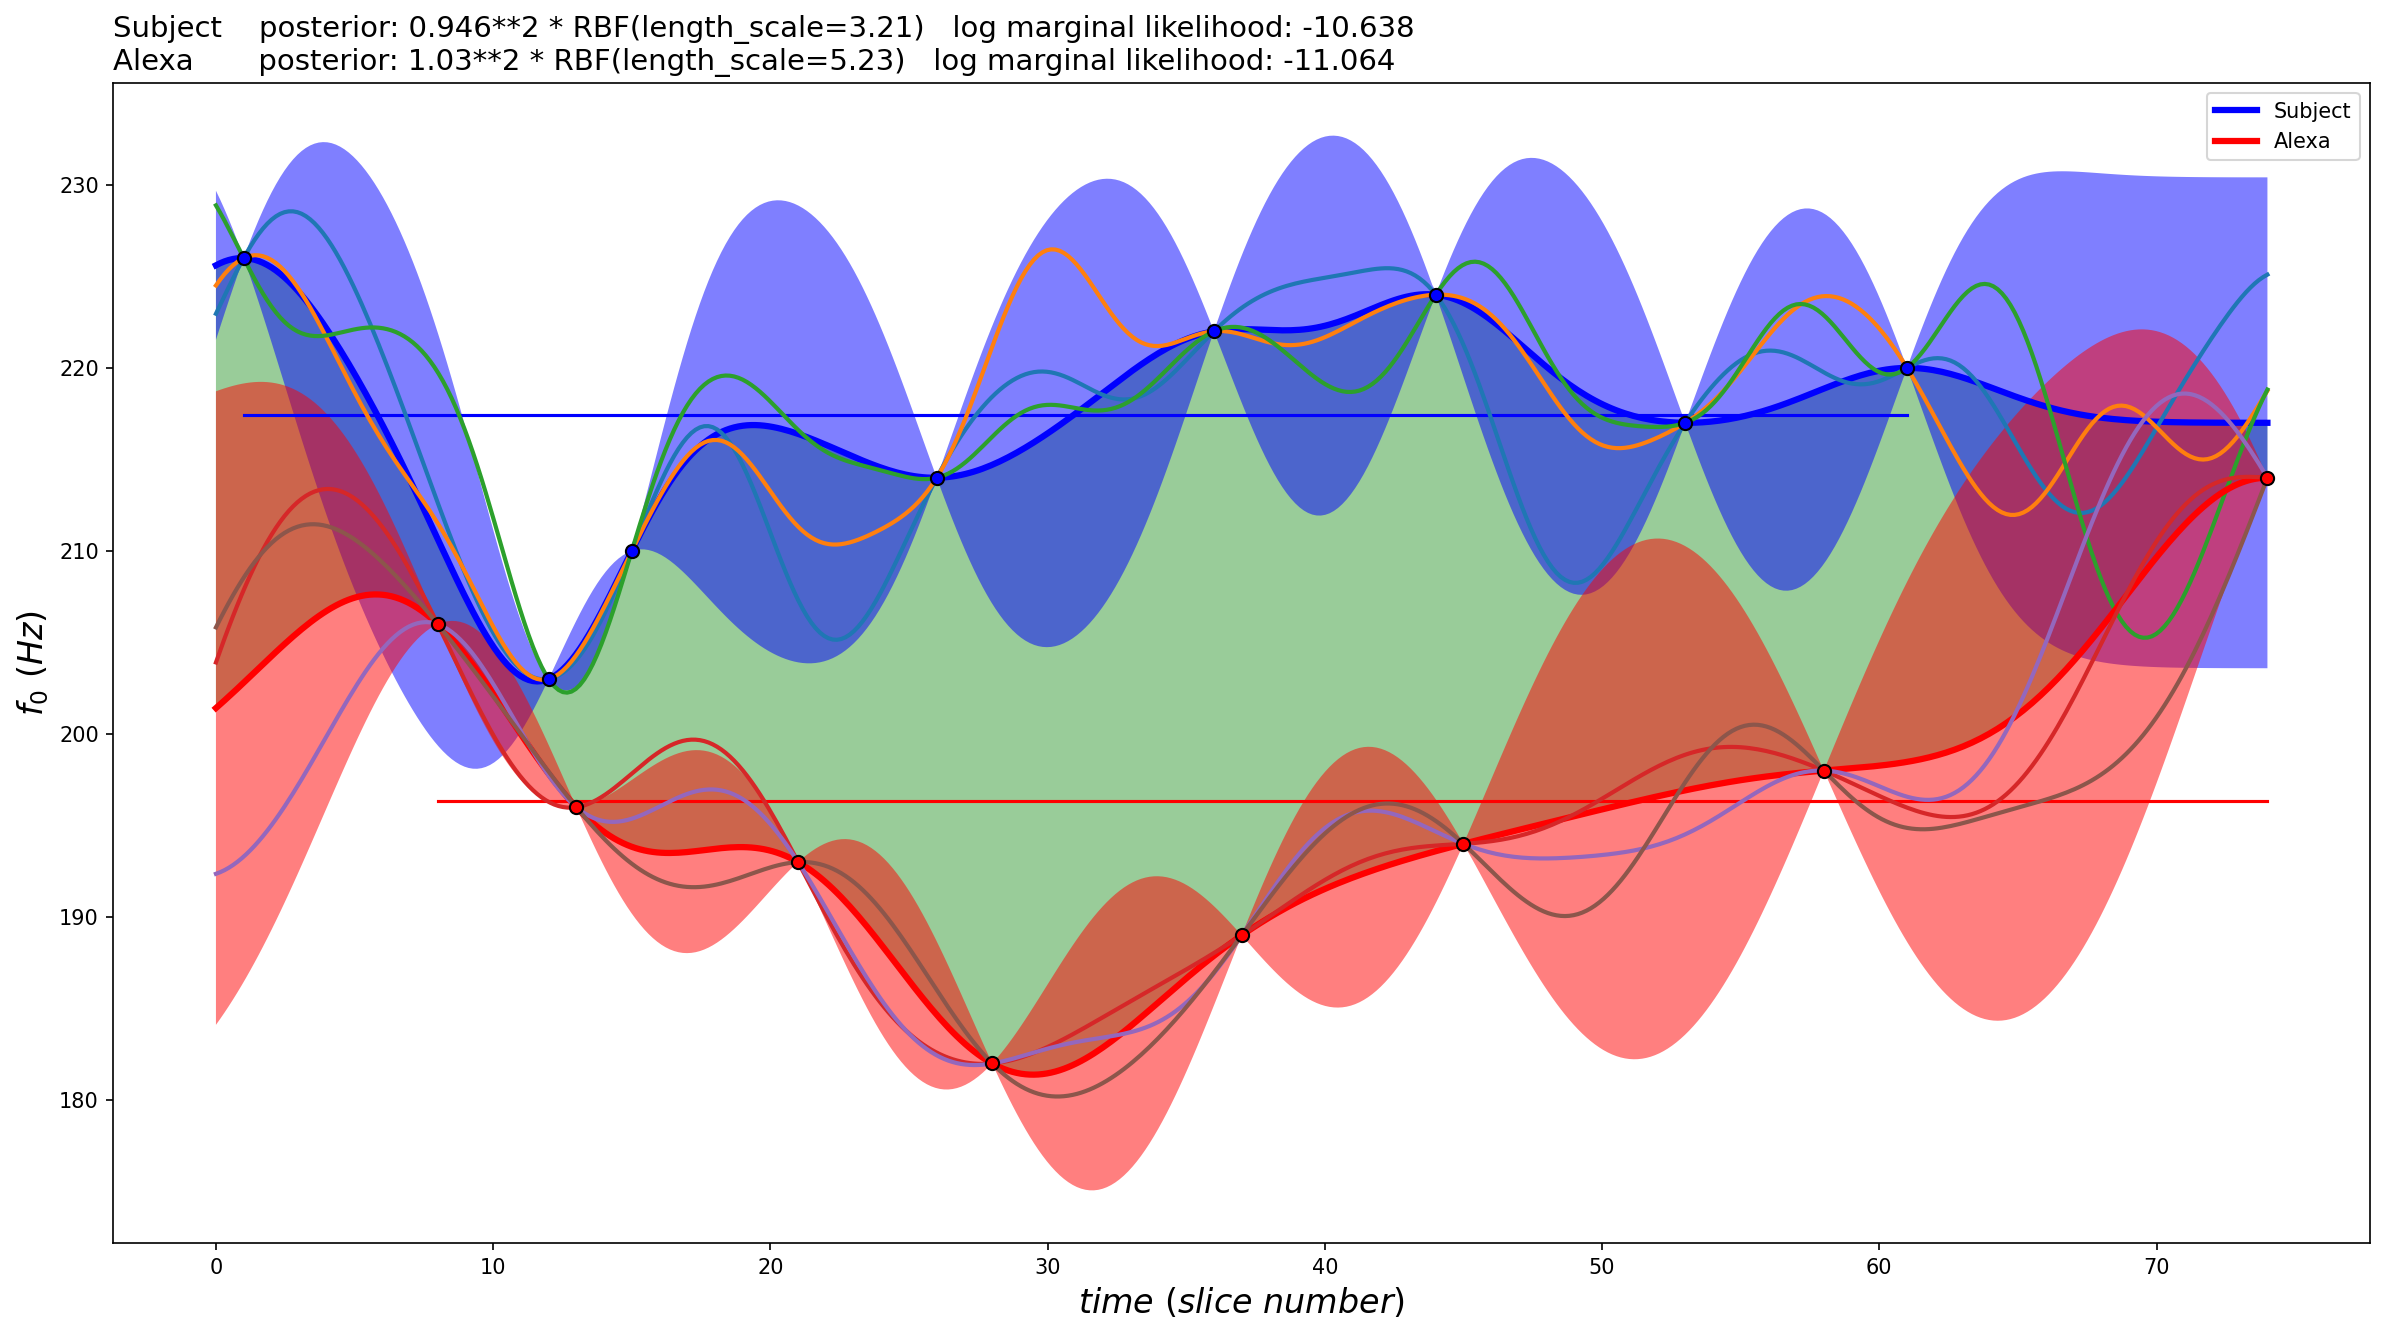
\includegraphics[width=\textwidth]{GP_VACC_with_draws}
	\caption[Gaussian process regression on a conversation with Alexa]
		{Gaussian process regression for an interaction of a subject with Alexa.
		 The thick blue and red lines show the predictions' mean.
		 The additional lines around the means are randomly drawn functions from the fitted kernel representing potential variational output.
		 The colored areas around the means lines show the \SI{95}{\percent} confident interval for the distributions of the same color.
		 The straight horizontal lines indicate the overall mean of each speaker's productions.
		 The posterior parameters and the log marginal likelihoods of the fitted distributions are stated at the top.}
	\label{fig:gp_vacc}
\end{figure}

\section{Marking degrees of change}
\label{sec:measuring_changes}

Once a regression line is drawn for each speaker from their respective distributions, the differences between the speakers' productions can be measured.
Furthermore, due to the higher temporal resolution, more fine-grained degrees of change over time can be calculated as well.
The differences are calculated by the subtracting the trapped areas between the two regression lines (see \cref{fig:gp_vacc})
%
\begin{equation}
	f_{diff} \equiv\Delta\vec{x}_* =
	\int_{\vec{x}_i}^{\vec{x}_{j}}\mu_{f_*subject} -
	\int_{\vec{x}_i}^{\vec{x}_{j}}\mu_{f_*alexa}
\end{equation}
%
and the directional derivatives of the resulted delta line to measure the degree of change
%
\begin{equation}
	\nabla\Delta\vec{x}_*' = \frac{d}{dx}f_{diff}
\end{equation}
%
along the delta line.
\Cref{fig:diff_and_derivatives} demonstrates this on the same conversation from \cref{fig:gp_vacc} using the mean predictions of each speaker.
%
\begin{figure}[t]
	\centering
	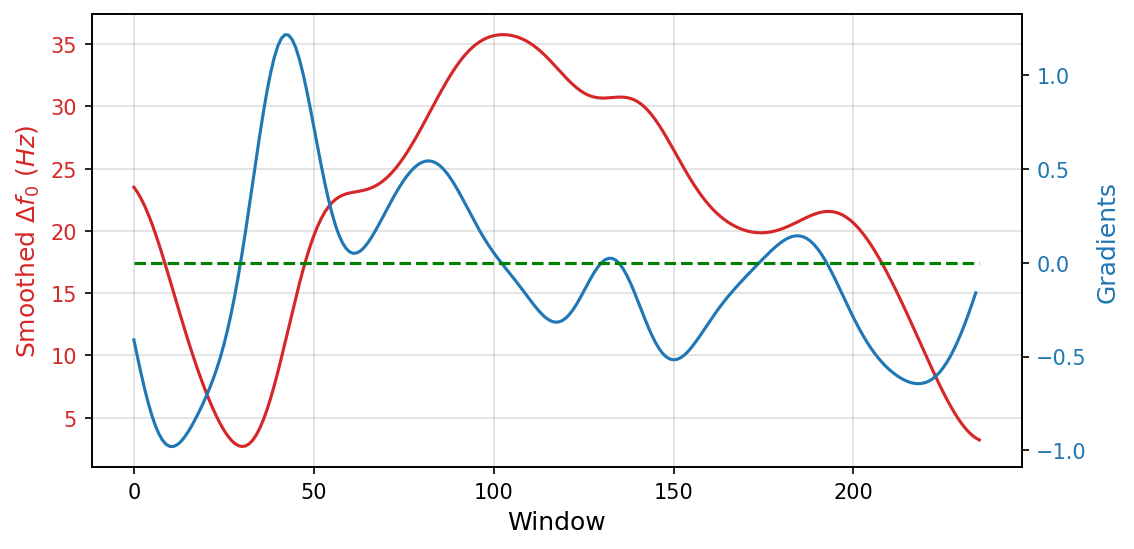
\includegraphics[width=\textwidth]{diff_and_derivatives}
	\caption[Continuous integral differences and derivatives in a \acl{hci}]
		{Continuous integral differences (red line) and their corresponding derivatives (blue line) of speakers' productions in a conversation.
		 The dashed green line shows the zero-gradient, , i.e., no change, threshold.}
	\label{fig:diff_and_derivatives}
\end{figure}
%
For building a generative model as described in \cref{sec:accommodation_as_a_lm,sec:clustering_and_incremental_generation}, the changes must be marked with pre-defined labels.
To that end, the derivative values were translated into a continuum of change ranging from \textit{divergence} to \textit{convergence}.
Based on this continuum, a discrete scale can be defined.
The more categories this discrete scale offers, the more specific the behavior descriptions can be.
\Cref{fig:cont_disc_scales} shows this process for a discrete scale of three categories: divergence, no (major) change, and convergence.
%
\begin{figure}[t]
	\centering
	\subfigure[Continuous scale]
		{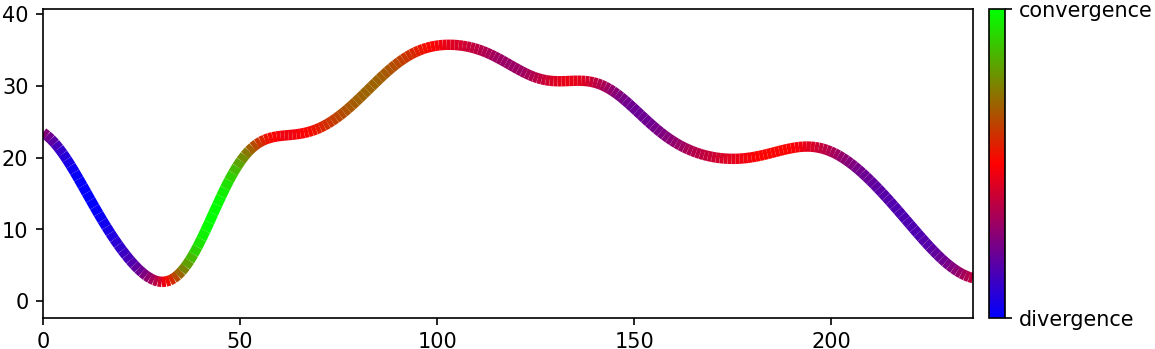
\includegraphics[width=0.47\textwidth]{cont_scale}
	\label{fig:continuous_scale}}
	\hfill
%	\vspace{-1cm}\hfill\hspace{-1cm}{\hbox{\LARGE $\Longrightarrow$}}\hfill
	\subfigure[Discrete scale]
		{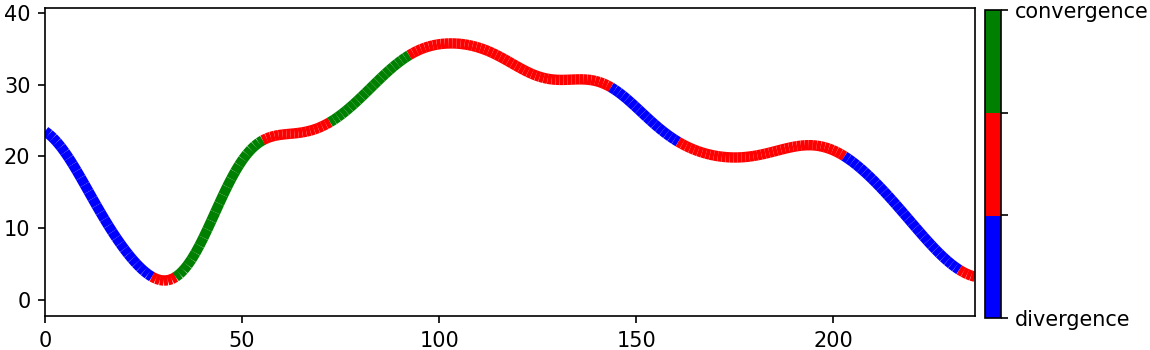
\includegraphics[width=0.47\textwidth]{discrete_scale}
	\label{fig:discrete_scale}}
	\caption[Continuous and discrete scales for labeling degrees of change]
		{Continuous and discrete color-coded scales for labeling degrees of change in a conversation.}
	\label{fig:cont_disc_scales}
\end{figure}
\todo[inline]{need more details regarding how the discrete categories are defined?}

\section{Accommodation as a language model} % Accommodation as an n-gram model
\label{sec:accommodation_as_a_lm}

In order to generate accommodation sequences, a model is needed, which can iteratively emit labels based on the label history. 
Predictions of any model based on Markov decision process \citep{Bellman1957markovian} depend only on the current state of the conversation.
This neglects any temporal aspect of the conversation, which is a key component in spoken dialogue and accommodation (see \cref{subsec:limitations_of_did,sec:crqa,sec:analysis_hhci}).
One way to overcome this is to extend the transition function of a Markov-based model, so that the previous $n$ states are somehow incorporated into the action $a$ of $P_a(s, s')$.
However, this violates the core idea of a Markov decision process and makes it cumbersome to use.
Therefore, an n-gram model is proposed here, which incorporates a portion of a sequence's history (\emph{context}) into the decision making, without losing the Markov property.
The estimation of the element $e$ at position $i$ is therefore calculated by the probability term $P(e_i \mid e_{i-(n-1)},\ \ldots\ , e_{i-1})$.
N-gram models are traditionally used for describing sequences of some linguistic units, e.g., words in a language model \citep[e.g.,][]{Niesler1996variable}, and are used in applications like machine translation \citep{Marino2006ngram} and proteins identification \citep{Xu2015identification}.
The n-grams model here describes sequences of \emph{accommodation levels} in a conversation.
These levels are represented by discretized values that are based on the degrees of change acquired in \cref{sec:measuring_changes}.
After computing the n-grams probabilities of the level, this model can be used for generating new sequences.
The resolution and variability of the model can be controlled by changing the n-grams' $n$ and the number of levels used to distinguish between the different accommodation levels.

\subsection{Dimensionality reduction and symbolic representation}
\label{subsec:dim_reduction_and_symbolic_rep}

The time series gradient extraction process described in \cref{sec:measuring_changes} (and see \cref{fig:diff_and_derivatives}) is greatly high dimensional, even for short interactions.
While this representation is useful for gaining a fine-grained overview of the data, it is not practical for various analysis techniques that do not benefit from (or are not designed to handle) such high dimensional data.
For instance, clustering algorithms, which need to iteratively compare between all points in a collection, scale better with lower dimensionality.
The dimensionality of the data in question here is reduced using \acf{paa} \citep{Keogh2001dimensionality}, which is a common dimensionality reduction technique for time series.
Each element $\vec{x}_i$ of the reduced vector is calculated by
%
\begin{equation}
	\label{eq:paa}
	\vec{x}_i = \frac{N}{n} \sum_{j=\frac{n}{N}(i-1)+1}^{i(\frac{n}{N})} S_j,
\end{equation}
\eqname{\Acl{paa} dimensionality reduction}\noindent
%
where $n$ is the dimensionality of the original times series, $1 \leq N \leq n$ is the dimensionality of the output vector, and $S_j$ is the $j$\textsuperscript{th} element of the original time series.
\Ac{paa} is suitable here, as the goal is to obtain vectors with fewer dimensions that still faithfully represent the data, and not, e.g., decompositions of the original data \citep[cf.\ method survey in][pp.\ 271-275]{Keogh2001dimensionality}.
As the goal here is to compare \emph{trends in change} within and across conversations rather than their absolute values, all gradient time series where z-normalized before applying the \ac{paa}.
In the context of conversation analysis, the \ac{paa}'s dimensional cardinality determines the \enquote{zoom} level, i.e., how fine-grained the representation is (the more points the more in detail the time series is described).
Ultimately, \ac{paa} provides \textbf{continuous numeric values} that represent the overall shape of the original time series.
\Cref{fig:paa} illustrates \ac{paa} on the gradients of one of the interactions.

\begin{figure}[t]
	% 20171130A_Quiz_01 was used for these figures
	\centering
	\subfigure[\acs{paa} based on the original time seires.
			   The blue continuous line shows the original time series representing the mutual change gradients in a conversation, which was extracted as described in \cref{sec:measuring_changes}.
			   The organe circles show the \acs{paa} points created based on the continuous lines.
			   The dashed orange line is the linear interpolation between the \acs{paa} points.
			   Note that this lines is for illustration only and is not taken into account for any \acs{paa}-related analysis.]
		{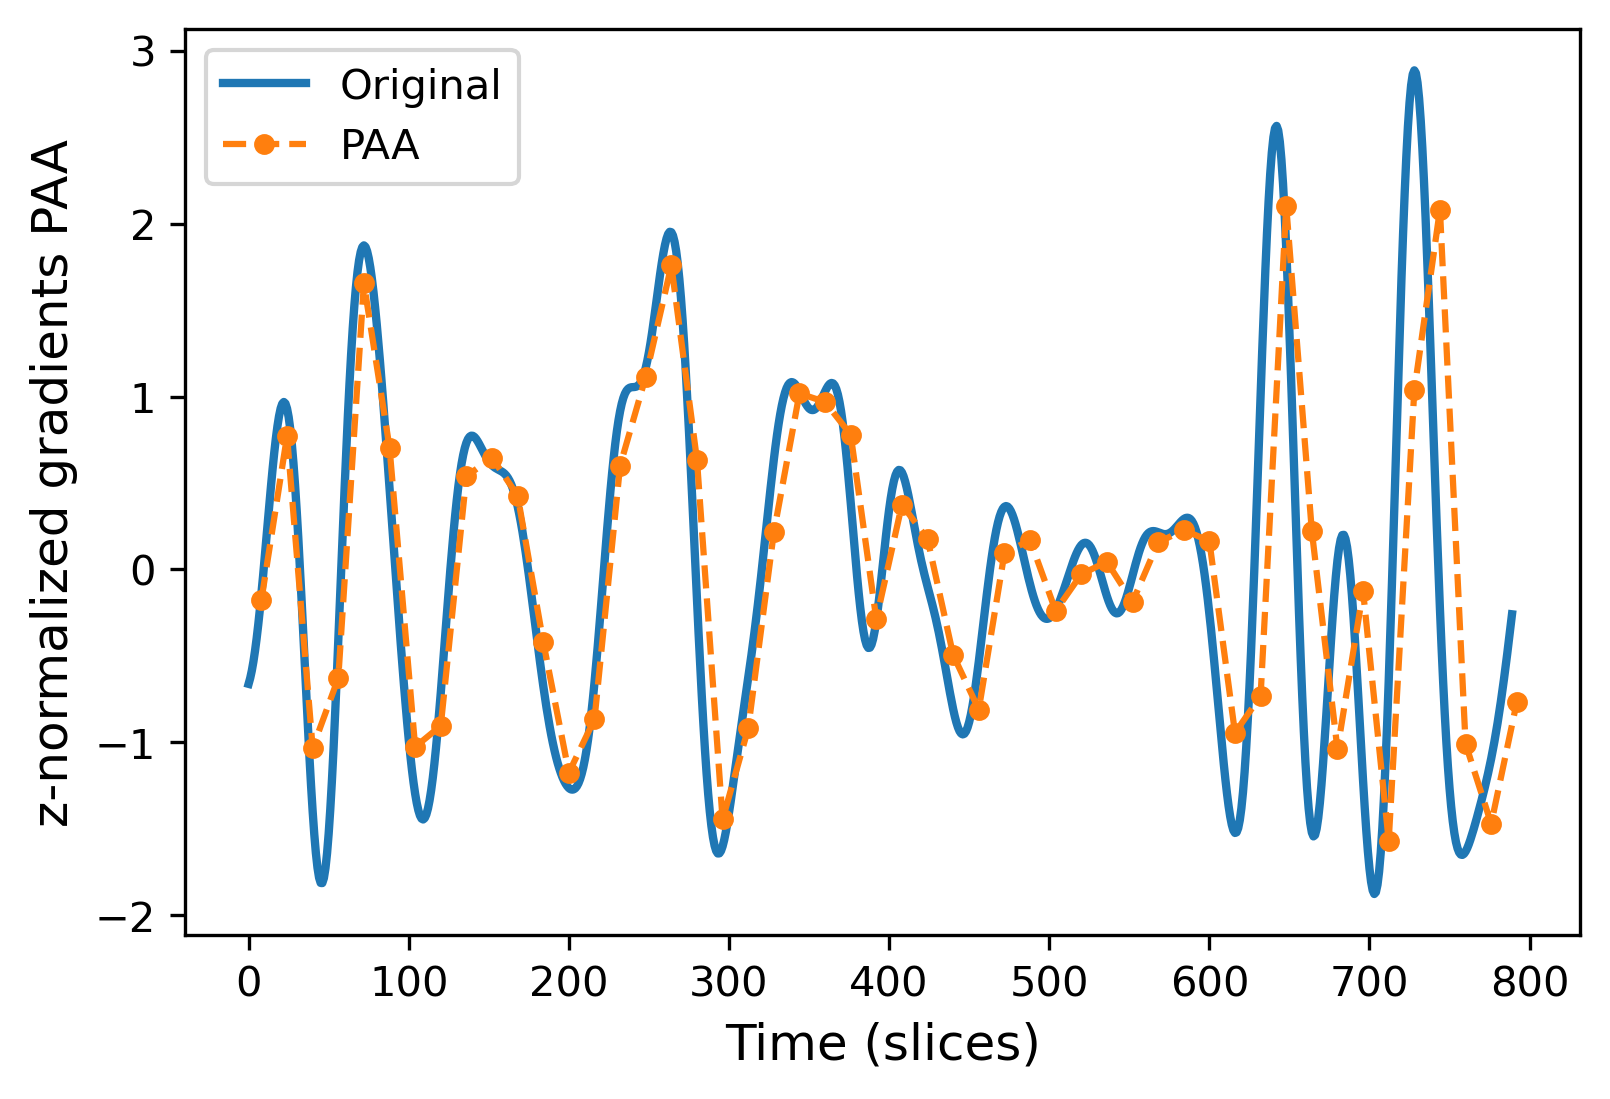
\includegraphics[width=0.47\textwidth]{PAA}
	\label{fig:paa}}
	\hfill
	\subfigure[\acs{sax} based on the \ac{paa} values.
			   The blue circles are the \acs{paa} points from \cref{fig:paa}.
			   The blue line visualizes the linearly interpolated trend of these points.
			   The horizontal green dashed lines show the margins of the five bins that split the points discrete categories derived from a normal distribution.
			   The organe labels (\enquote*{d+}, \enquote*{d}, \enquote*{n}, \enquote*{c}, and \enquote*{c+}) mark the classification of each point based on the bin it falls into.]
		{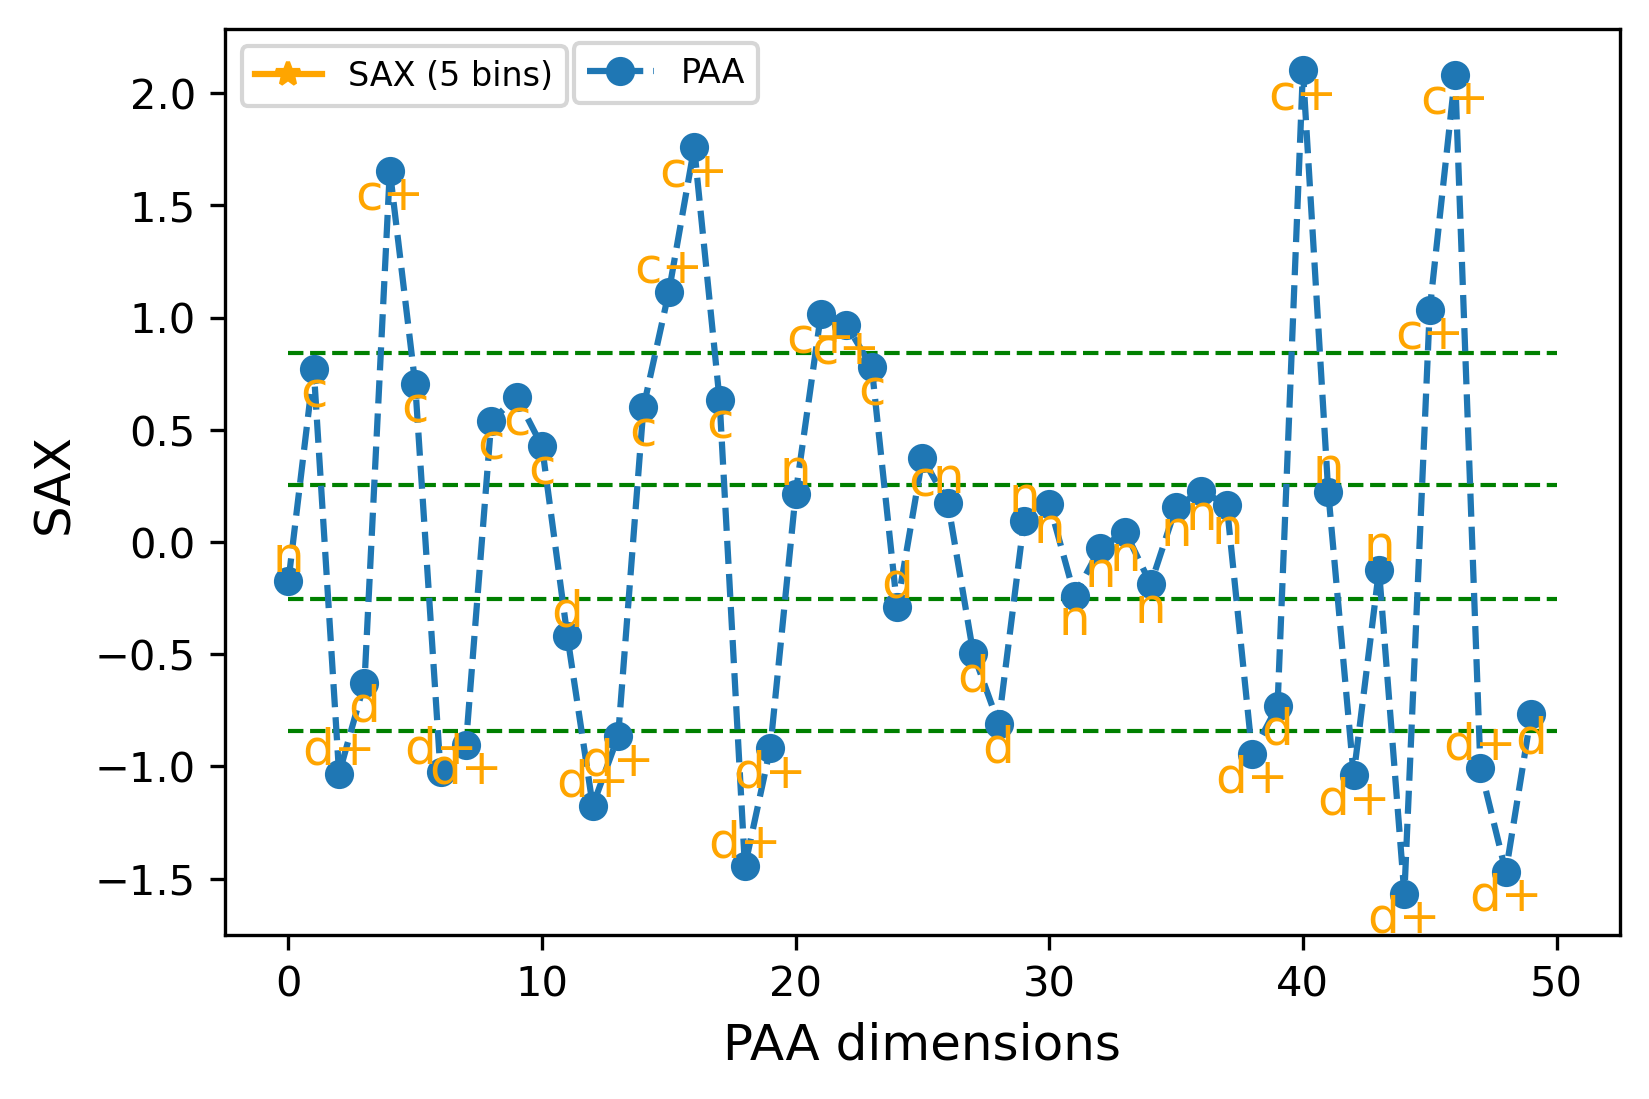
\includegraphics[width=0.47\textwidth]{SAX}
	\label{fig:sax}}
	\caption[\Acl{paa} and \acl{sax} for the time series representation of mutual change in a conversation]
		{\Ac{paa} and \ac{sax} for the time series representation of mutual change in a conversation.}
	\label{fig:paa_and_sax}
\end{figure}

\Ac{paa} is suitable for analyses of continuous numeric values.
However, discrete values are required for symbolic sequence-based processing, such as calculating probabilities of n-grams.
For converting the continuous \ac{paa} values, the \acl{sax} \citep[\acs{sax};][]{Lin2007experiencing} method was used.
\Ac{sax} assigns a string label to each of the pre-defined bins.
This is an advantage of \ac{sax}, as these labels provide a more meaningful and intuitive representation.
As explained, e.g., by \citet{Apostolico2003monotony}, it is preferable to use a discretization technique that outputs a symbol set with equiprobability\footnote{It can be claimed that realistically equiprobability does not hold for the symbols in this kind of data.
While that may be true to some extent, neither the pre-processing nor the dimensionality reduction steps held any assumptions regarding the values in each \ac{paa} sequence.
Moreover, the data was z-normalized to avoid any bias stemming from specific numeric values.
For these reason, together with the fact that the participants were, in practice, free to speak in whatever way they wanted, equiprobability can be assumed in this analysis.
See \cref{subsec:word_extraction_and_seq_prob} for more information regarding the distribution of extracted symbol sequences}.
To that end, the \ac{sax} discretization was done using bins based on the normal distribution of the values.
% this is defined by the method="normal" parameter in the SAX function (or `strategy` parameter internally)
Five categories (bins) are used here for categorizing degrees of change, labeled \enquote*{d+} for \emph{strong divergence}, \enquote*{d} for \emph{divergence}, \enquote*{n} for \emph{no (major) change}, \enquote*{c} for \emph{convergence}, and \enquote*{c+} for \emph{strong convergence}.
This number of bins was found to adequately describe types of accommodation;
three categories resulted in too unspecified sequences where all degrees of convergence or divergence are labeled similarly (as in \cref{fig:discrete_scale}), and seven or more categories did not add a substantial added value and often yielded sparse sequences.
The motivation for choosing an odd number of categories is to have a neutral (\enquote{no-change}) category.
However, an even number can be used as well, forcing each value to stand for either convergence or divergence while ignoring zero values.
Note that the term \emph{synchrony} is avoided here for describing a steady distance between the speakers, because per its definition introduced in \cref{subsec:variation_types}, it entails additional properties.
Ultimately, \ac{sax} provides \textbf{discrete textual labels}, which are a discretized version of the original time series.
\Cref{fig:sax} shows the \ac{sax} of mutual change time series based on the \ac{paa} points in \cref{fig:paa}.

\subsection{Sequence extraction and probability calculation}
\label{subsec:word_extraction_and_seq_prob}

After applying \ac{sax}, a sequence of accommodation labels is obtained for each corresponding interaction.
The count distribution of the labels was computed to examine their frequency.
As could be expected, the symbol $n$ had the highest frequency.
This frequency was about 2.5 times higher than the convergence and divergence labels $c$ and $d$, whose frequency, in turn, was roughly four times higher than the frequency of the strong convergence and strong divergence labels $c+$ and $d+$.
The same calculations were repeated for combinations of the labels as they appear in the \ac{sax} sequences.
The frequencies can be separated into three groups:
Matching the trend of the single-label distribution, repeated $n$ labels were about three times more frequent than the second group, which consisted of most other combinations that included $n$.
Lastly, this group was followed by a long tail of less frequent sequences, starting from counts three to four times lower, which included the rest of the symbol combinations.
Sequences with many repeated $c+$ or $d+$ labels (i.e., sustained convergence/divergence) mostly appeared toward the end of the tail.
Increasingly smoother instances of the same overall distribution shape were found for all sequence lengths from two and up to half the \ac{sax} sequence length (after which such frequencies become not as meaningful).
The percentage of covered n-grams of length $w$ found in the \ac{sax} sequences out of the $5^w$ theoretically possible combinations was exponentially lower the higher $w$ was.

\begin{table}[t]
	\centering
	\caption[Examples of probabilistically generated accommodation level label sequences]
		{Three examples of probabilistically generated accommodation level label sequences.
		 Each sequence consists of eight labels that were generated based on the initial context of the padding symbol $p$.
		 The first line of each example shows the generated symbols as introduced in \cref{subsec:dim_reduction_and_symbolic_rep} and their average variability (value between 0 and 1, higher number means more variability.).
		 The second line lists the scores (probabilities) of each corresponding generated label given the context seen up to that point and the overall probability of generating this entire sequence.
		 The third line lists the perplexity of the trigram ending with the corresponding generated label given the context at the time of the generation.
		 Note that the first two padding labels do not have score values, as they are given as the initial context.
		 Similarly, perplexity can only be calculated once the sequence is longer than the one trigram.}
		 % variability was calculated as the average "deviation", where c and d have value of 0.5, c+ and d+ value of 1, and n value of 0. for Example (c + c+ + n + n + d+ + c + n + n) / 8 = 0.375
	\label{tab:generated_symbol_sequences}
	\begin{tabularx}{\linewidth}{*{10}{c}l@{\hskip 0.1cm}l}
		\toprule
		p    & p    & n    & n    & n    & c    & n    & d    & d    & c    & variability: & \num{0.187}  \\
		---  & ---  & 0.44 & 0.46 & 0.55 & 0.18 & 0.32 & 0.29 & 0.25 & 0.35 & probability: & \num{1.63e-4}\\
		---  & ---  & ---  & 2.22 & 1.99 & 3.16 & 4.16 & 3.27 & 3.67 & 3.35 & perplexity: & \num{3.11}   \\[0.4cm]
		
		p    & p    & n    & d    & d    & c    & c+   & d+   & d+   & c+   & variability: & \num{0.687}  \\
		---  & ---  & 0.44 & 0.17 & 0.25 & 0.35 & 0.13 & 0.25 & 0.34 & 0.19 & probability: & \num{1.37e-5}\\
		---  & ---  & ---  & 3.67 & 4.88 & 3.35 & 4.69 & 5.62 & 3.46 & 3.96 & perplexity: & \num{4.23}   \\[0.4cm]
		
		p    & p    & c    & c+   & n    & n    & d+    & c     & n    & n    & variability: & \num{0.375}  \\
		---  & ---  & 0.30 & 0.25 & 0.25 & 0.16 & 00.04 & 00.20 & 0.22 & 0.41 & probability: & \num{2.16e-6}\\
		---  & ---  & ---  & 3.67 & 4.03 & 5.02 & 12.72 & 11.51 & 4.77 & 3.30 & perplexity: & \num{6.43}   \\
		\bottomrule
	\end{tabularx}
\end{table}

N-grams of $n = 3$, i.e., trigrams, are used here for computing the label probabilities.
The size of the n-gram determines the amount of previously acquired evidence taken as context when calculating the probability of the a subsequent label.
This fulfills the same role as the \emph{pool size} parameter of the computational model (see \cref{sec:parameters}).
In both cases, the goal is to consider the temporal evolution of the conversation for deciding on its continuation.
To account for conversation-initial sequences, the beginning of each symbol sequence is padded.
The end of the sequence is not padded, since, unlike a traditional language model, the generative model here lets the user decide on the end of the interaction (see \cref{sec:clustering_and_incremental_generation}) and therefore does not attempt to predict it.
This summed up to a collection of \num{2700} trigrams, which comprised 143 out of the $5^3$ level combinations~+~1~$\times$~5~two-padding combinations~+~5~$\times$~5~one-padding combinations~$= 155$~possible symbol combinations (\SI{92}{\percent}).
% 2700 is 54 solo interactions times 50 trigrams for each: the size of SAX used was 50, which gives 48 trigrams. with the 3 trigrams added from padding, it's 50. 50 times 54 = 2700
This shows a great variety of conversation dynamics.
% however, since not all possible combinations are used for training, unseen trigrams can still be seen during generation. we set the vocab to be all possible combinations (plus all initial padded trigrams)
% smoothing??
% probabilities for OOV trigrams?
Based on this n-grams model, sequences of symbols, representing accommodation levels in a conversation, can be probabilistically generated.
For example, the next accommodation level $l$ after two convergence labels $c$ is taken from the probability distribution $p(l \mid c,\ c)$.
\Cref{tab:generated_symbol_sequences} shows examples of such probabilistically generated sequences for the first eight accommodation labels of a conversation.
The variability measure is defined as
%
\begin{equation}
	sequence\ variability = \frac{1}{N} \sum_{i=1}^{N} \left| \frac{num(label_i)}{2} \right|,
	% the absolute value is divided by 2 to make the vaerage per turn (i.e., max 1 "variability point" per turn)
\end{equation}
\eqname{Label sequence variability score}
\noindent
%
where $N$ is the number of labels in the sequence and $num(label)$ maps a label to a numeric value between -2 ($d+$) and 2 ($c+$).
The overall probability of the sequence is calculated by
%
\begin{equation}
	sequence\ probability = \prod_{i=1}^{N} p(label_i \mid label_{i-2}, label_{i-1}).
\end{equation}
\eqname{Label sequence probability score}
\noindent
%
The perplexity measure is the average of all the individual perplexity scores of the labels in the sequence.
It is worth noticing that the third sequence in the table has lower variability than the second sequence, although its overall probability is lower and its mean perplexity is higher.
That means that, based on this model, interactions with lower variability are not necessarily more likely.
On the other hand, since in most contexts, the probability of label $n$ is relatively high, sequences with many $n$ labels are more likely to appear, on average.

\section{Clustering and incremental variational generation}
\label{sec:clustering_and_incremental_generation}

After defining a unified representation of the mutual changes in interactions over time in \cref{subsec:dim_reduction_and_symbolic_rep}, the question arises whether clusters can be found in these representations to detect general similarities in behavioral patterns.
Two clustering methods are used for that, namely \ac{knn} and hierarchical linkage, each offering a different angle and insights.
The former method is a top-down approach with a pre-defined number of clusters, which offer a more general view on the patterns, and the latter is a bottom-up approach with no prior assumptions, where more speaker-specific differences can be measured.
While it cannot be expected to find a completely distinct pattern for each speaker, some separable clusters and general tendencies are expected to emerge, both when inspecting individual speakers and the collection as a whole.
%
\begin{figure}[t]
	\centering
	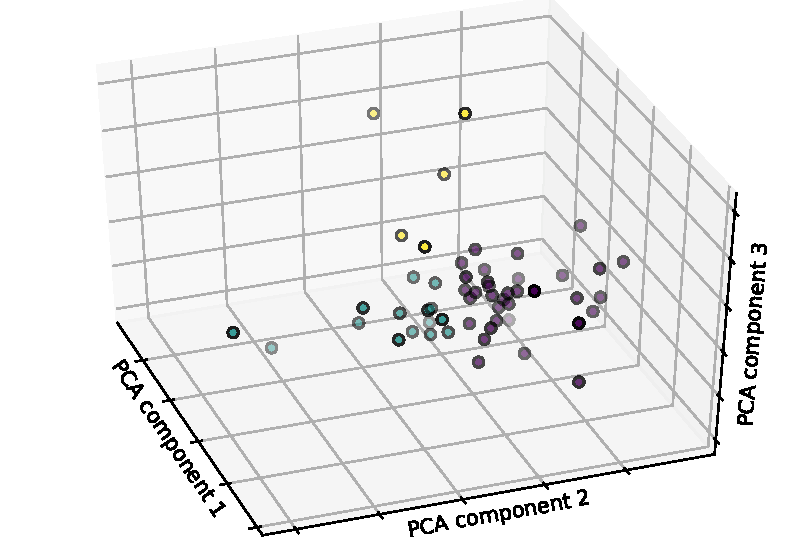
\includegraphics[width=\textwidth]{3d_clustering}
	\caption[3D \ac{knn} clustering of mutual changes \acs{pca} components]
		{\ac{knn} clustering of the first three \ac{pca} components of the interactions' \ac{paa} sequences.
		 Each circle represents one sequence in the three-dimensional space.
		 A circle's color indicates the cluster to which the datapoint belongs.}
		 % elevation is 40 azimuth is 160
	\label{fig:knn_clustering}
\end{figure}
%
For \ac{knn} algorithm was used for clustering, the process was performed with two, three, and five clusters using the two or three first \ac{pca} components, with the combination of three clusters and three components performing the best on average.
Since the \ac{paa} representations created in \cref{subsec:dim_reduction_and_symbolic_rep} can be arbitrarily long and high dimensional, they are reduced here to their $n$ first \ac{pca} components for visualization purposes.
% on average since kNN is not deterministic and was run multiple times
The result is shown in \cref{fig:knn_clustering}.
\todo{need references for PCA and kNN?}

\begin{landscape}
	\begin{figure}[t]
		\centering
		\hspace*{-4cm}
		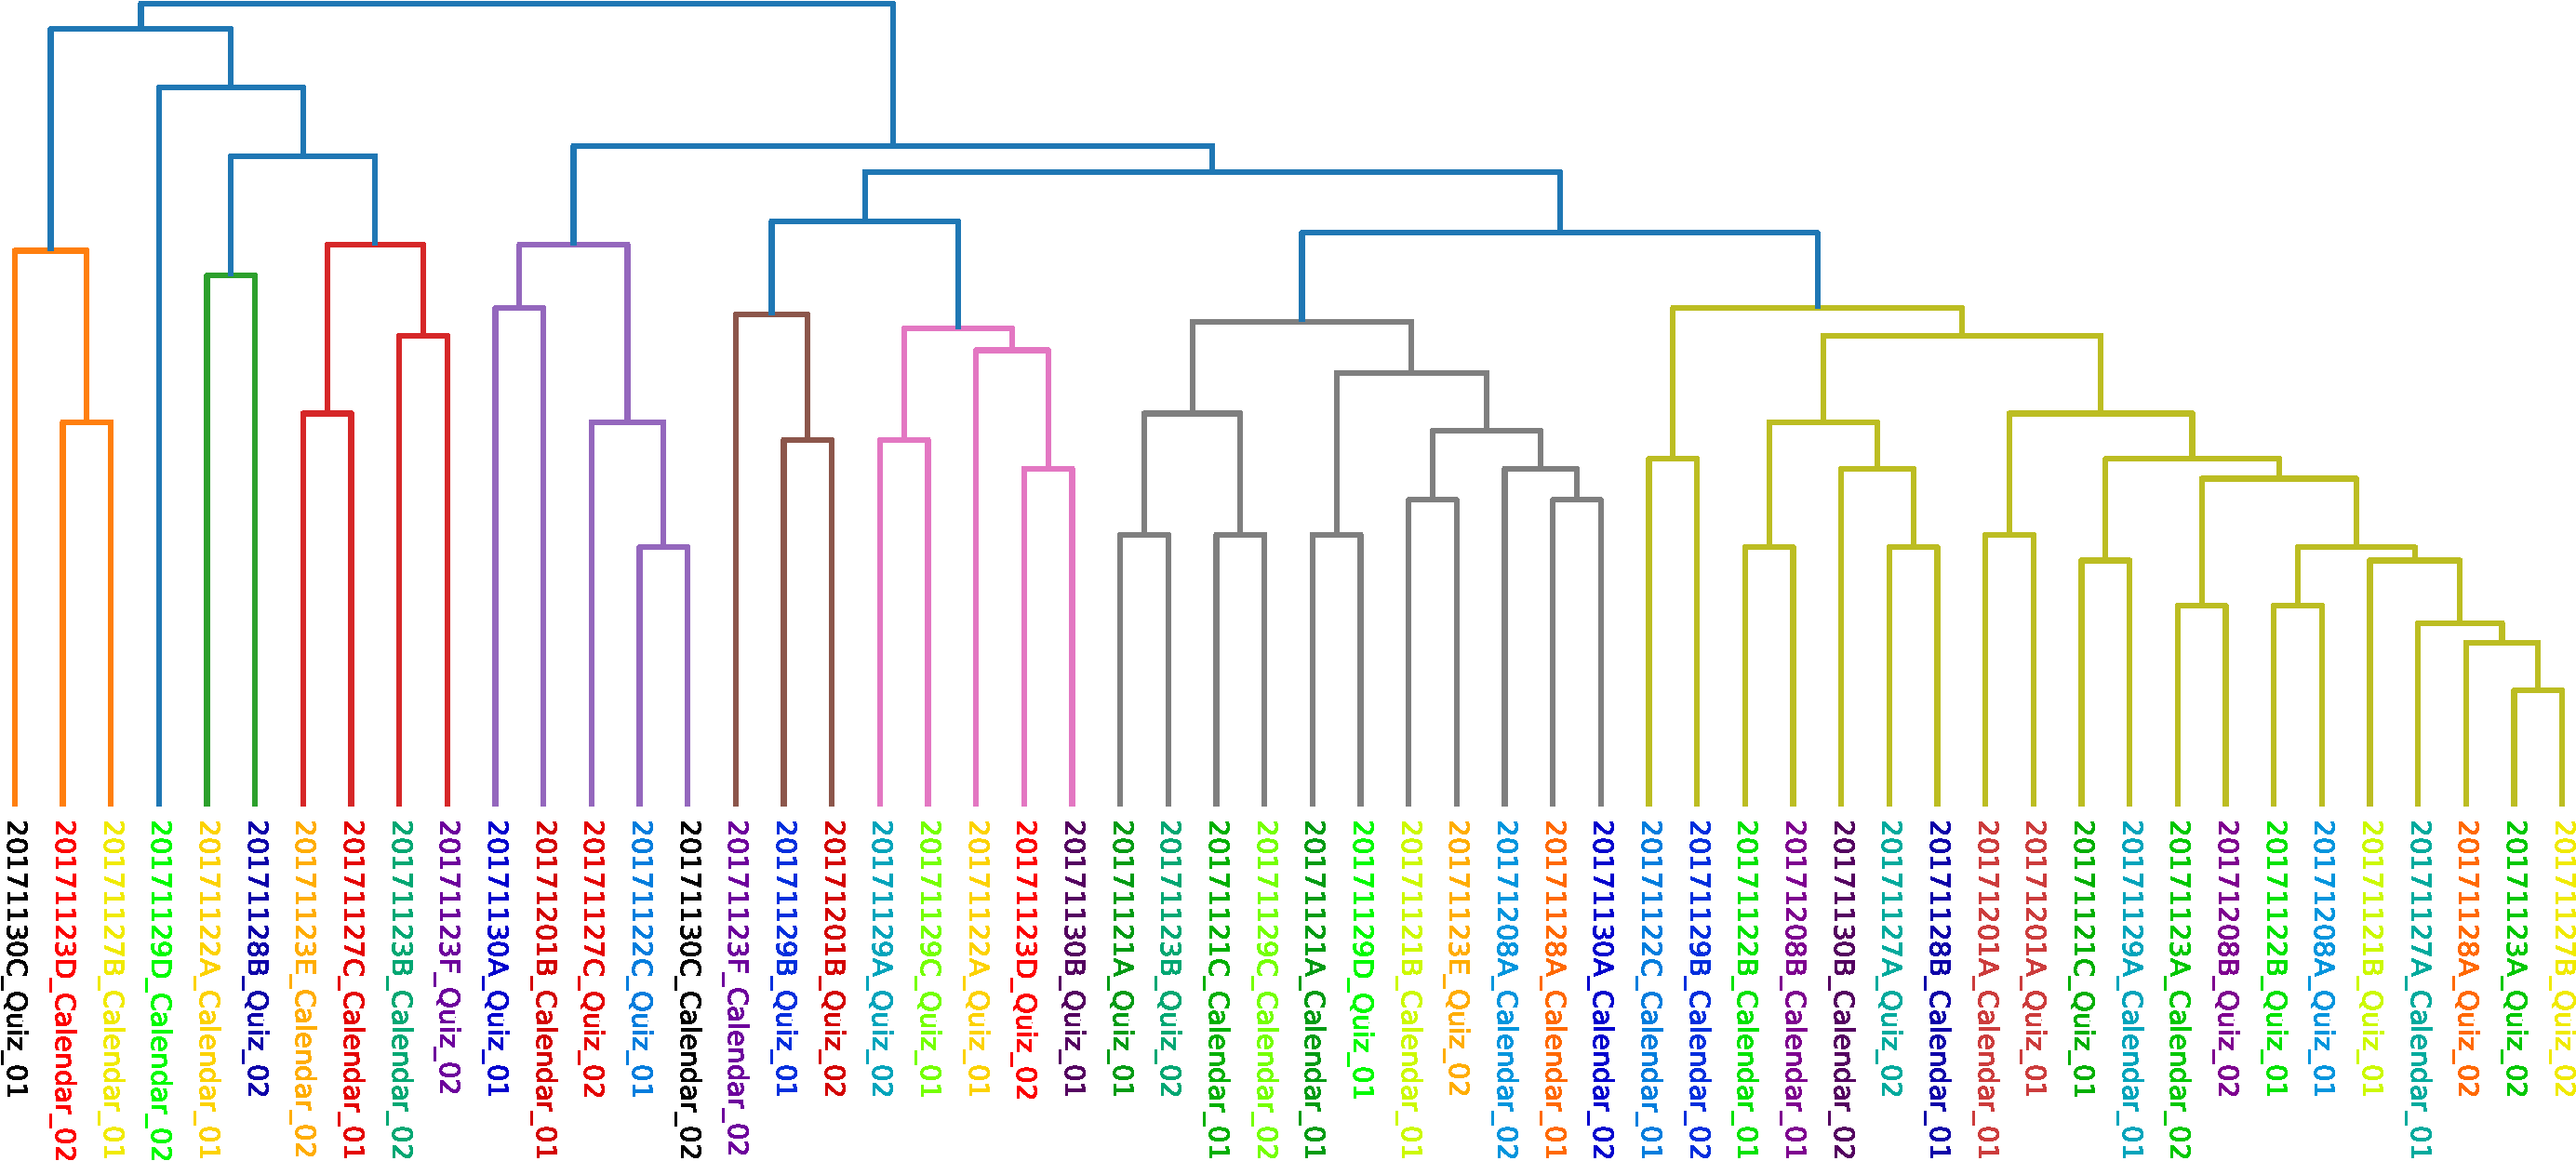
\includegraphics[width=1.7\textwidth]{paa_dist_dendrogram}
		\caption[Dendrogram of time series representation of interactions distances]
			{Dendrogram of the time series \ac{paa} representations of the solo condition interactions based on complete-link distances.
			 Each cluster is represented by a different color of lines.
			 Blue lines connect pairs of clusters that are most similar to each other, and similarly pairs of the closest subsequent sub-cluster and eventually leaves are connect directly to each other.
			 Each leaf represent the interaction indicated by its label.
			 Labels of the same color mark interaction with the same subject (two interactions per subject).
			 The leaf and cluster colors are \emph{not} related.
			 The leaves are order horizontally by their distance from left to right, so that the leaves of interactions that are more similar to each other (both inter- and within-cluster) are positioned closer.
			 For example, the two interactions of subject \emph{20171201A} (12\textsuperscript{th} and 13\textsuperscript{th} leaves from the right) are the closet to each, as they are positioned together and within the same smaller sub-cluster.}
		\label{fig:paa_dist_dendrogram}
	\end{figure}
\end{landscape}

While top-down clustering can uncover general grouping of elements, bottom-up hierarchical clustering can reveal structural relations between them and measure their degrees of similarity.
The distances between the 54 interactions can be measured and compared using the \ac{paa} values.
The calculation was done using \emph{complete link} (a.k.a.\ farthest point algorithm) agglomeration technique.
This kind of linkage is supported by the assumption that there are more general behavior patterns beyond the individual differences, as it searches for the most dissimilar (and hence principally all) interactions in neighboring clusters and not only the closest one.
This method also allows using the entire \ac{paa} sequences without any pre-processing.
\Cref{fig:paa_dist_dendrogram} shows the bottom-up distance clustering based on this linkage. 
Although, unsurprisingly, no definite order emerges, some general trends can be seen regarding the similarity between interactions of the same human speaker.
As the leaves are ordered horizontally based on their overall similarity, the distances between their positions are utilized to determine each subject's behavior consistency.
The average distance of the population is 16.5, far from the maximal possible average of 27.
% This is the maximal possible average, since this is when each interaction is half of the population away from its pair.
% With the largest possible distance between two leaves being 53, the space can be divided into three bins of 18 (rounded up).
Dividing the space into three equal bins of \enquote{short}, \enquote{medium}, and \enquote{long} distances shows that 16, 10, and 1 interaction(s) fall into these bins, respectively.
Moreover, this distribution has a median of 16 and its second tertiles located at 19, far from the \enquote{long distance} bin.
Such skewness in the distribution indicates that interactions of the same speaker tend to be relatively similar in terms of accommodation trends, regardless of any other factor (interaction length, task, order, and other factors discussed in \cref{chap:speech_variations_in_hhci}).
Notably, the two interactions of one participant, 20171201A, even have the minimal possible distance of 1 between them (12\textsuperscript{th} and 13\textsuperscript{th} leaves in \cref{fig:paa_dist_dendrogram}) and they are in the same lower-level sub-cluster.

These clustering techniques show that different accommodative behaviors among speakers can be found and quantified.
Together with the probabilistic approach presented in \cref{subsec:word_extraction_and_seq_prob}, these can be used for generating sequences based on a specific behavior (or rather a group of latent behaviors).
Ultimately, this would result in a variational behavior of a system while interacting with a user (along with some a core latent behavior), as described in \cref{subsec:variation_types}.
To this end, an \emph{incremental} generation process is needed, as opposed to the generation process demonstrated in \cref{tab:generated_symbol_sequences}, where the data for the entire interaction was known, an incremental generation is introduced here.
An incremental generation better represents a live interaction, in which only the evidence accumulated up to a certain turn can be used for analysis and prediction of the next turn.
This can be utilized both for integration into a system and for simulating possible system behaviors for research.
%
\begin{figure}[t]
	\centering
	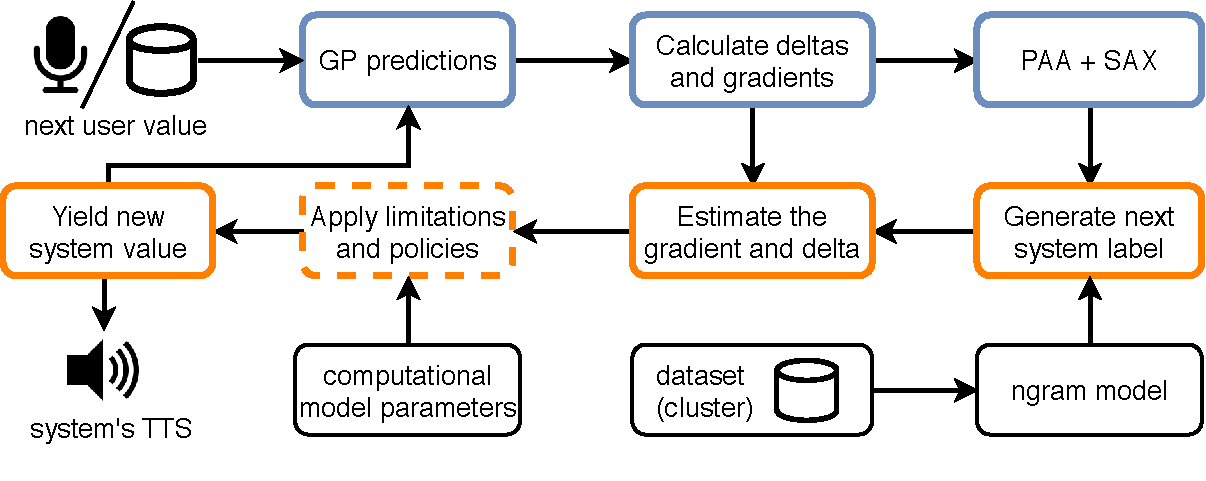
\includegraphics[width=\textwidth]{incr_gen_pipe}
	\caption[Incremental generation process]
		{Schema of the incremental generation process.
		 Blue boxes are related to the user phase and orange boxes to the system phase.
		 Together, they complete a cycle of one round.
		 The dashed orange frame marks an optional step.
		 Note that the new value generated for the system is used both as output (e.g., for \ac{tts} synthesis) and as additional evidence for the next cycle.
		 The user's values can be obtained either from online input or from some database.}
	\label{fig:incr_gen_pipe}
\end{figure}
%
The process is summarized in \cref{fig:incr_gen_pipe}.
It consists of the user and the system phases, which are roughly symmetric and with opposite goals:
While the former assigns a label to an input value, the latter yields a value based on a label (which, in turn, is generated based on the label assigned to the user's input).
A round is completed once both phases were executed once.
Hence, each round adds two values and their two corresponding labels, one for the user and one for the system.
In the user phase, the user input -- obtained either for live input or a database -- is added to the rest of the so-far accumulated evidence to predict both the user and the system values up to the current turn using \acp{gp} (the same way as in \cref{subsec:interploating_data_using_kriging}).
Then, deltas and gradients of these values are calculated (see \cref{fig:diff_and_derivatives}) to subsequently create \ac{paa} and \ac{sax} sequences (see \cref{fig:paa_and_sax}).
In the system phase, the resulted \ac{sax} contains one label per turn, including the user's new turn.
The next system label is generated using the n-gram model with the probabilities acquired from the subset with the desired accommodative behavior (a cluster from \cref{fig:knn_clustering} in the example below).
This label represents a relative z-normalized change degree.
Therefore, the value range covered by this label can be computed from all accumulated gradients (shown by the arrow between the second user step to the second system step in \cref{fig:incr_gen_pipe}).
The system's \ac{gp} from the first step, which holds the expected behavior, is used to draw a single gradient value from that range.
These two steps grant the variational property to the generation process; a label for the general accommodation direction and a value for the specific amount of change.
The drawn gradient value and the last system's gradient are used to determine the new gradient, from which the next system value can be calculated.
Importantly, external policies can intervene in this step and modify this value to enforce the desired change of the system (see \cref{subsec:assign} for more motivation and examples).
The yielded value is then added to the accumulated evidence, so that it can be taken into account in the next round.
In parallel, it can also be sent to a component of a \ac{sds} (e.g., the \ac{tts} module, see \cref{subsubsec:dialogue_system,fig:adaptation_module_architecture}).

\begin{figure}[t]
	\centering
	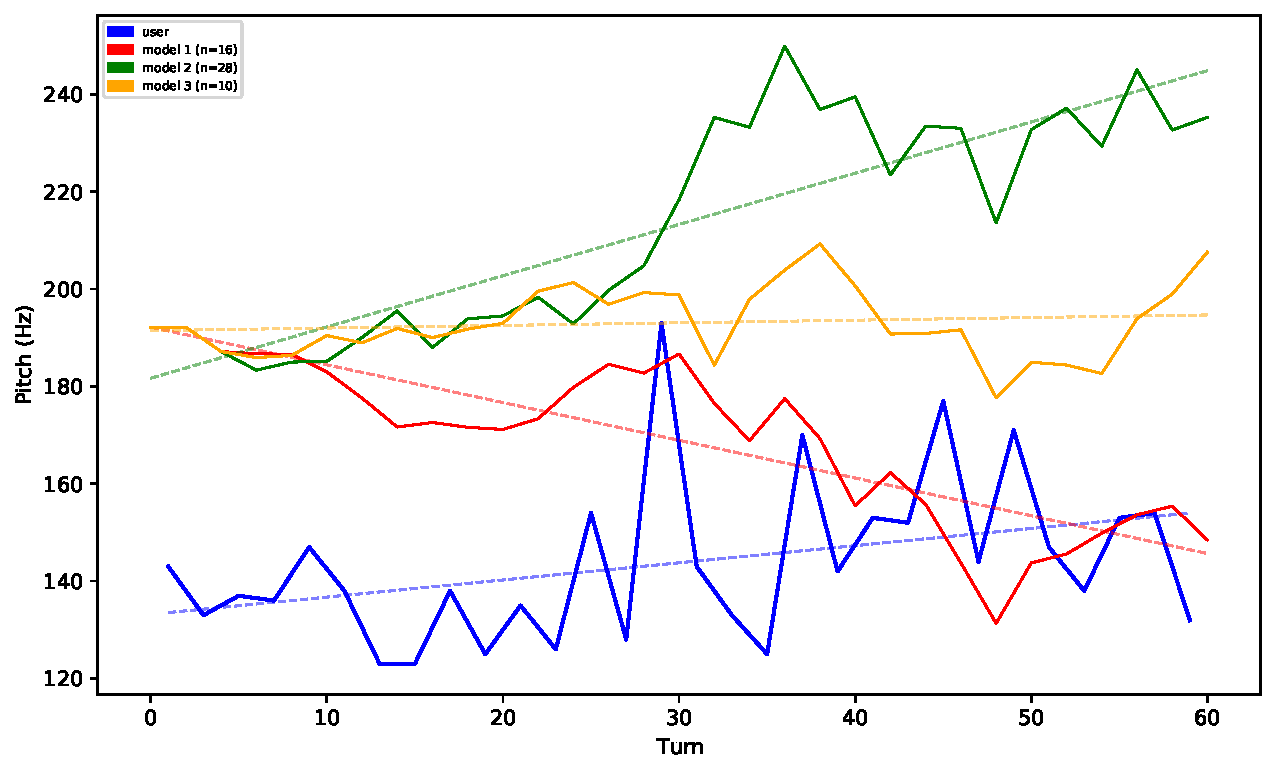
\includegraphics[width=\textwidth]{incr_gen_models}
	\caption[]
		{Responses of the three models, generated for the same user input (in blue).
	 	 The dashed lines show the linear overall trend of the solid line of the same color.
	 	 Note that these lines should be taken a reference for the general trend and \textbf{not as a representation or estimation of the values}.}
	\label{fig:incr_gen_models}
\end{figure}

This process was used to simulate accommodation changes during a conversation using the three clusters from \cref{fig:knn_clustering}.
Although the dataset used here is relatively small and is not designed to trigger different behaviors, the natural tendencies of the participants should be, at least to some extent, reflected in this latent representation and be expressed in these simulations.
For each cluster, an n-gram model was created as described in \cref{subsec:word_extraction_and_seq_prob}, based only on the interactions from this cluster.
These models were then used to generate an accommodation response for each turn, similarly to those shown in \cref{tab:generated_symbol_sequences}, but longer and with concrete values in addition to the labels.
However, this time the generation was only for the system's side, given a pre-defined input of a human use. simulating a live interaction.
In the example presented here, raw production values were used (from interaction \texttt{20171201B\_Calendar\_02}), but there is room for system designers to control this differently depending on the application.
For example, in interactions where the user is expected to take multiple turns before giving the floor to the system, only the last few values (as motivated in \cref{chap:conv_analysis}) or the average of these turns could be used instead.
The first 30 rounds (60 turns) of three hypothetical conversations for this input were generated, one per model.
An n-gram length of ten symbols was used, to take advantage of the longer context available in this longer interaction.
All the models start with the mean value of the system in the data, which would be known also in a real-world scenario from the development of the system's \ac{tts} component.
% and hence doesn't break the rule that only data available in a real live conversation is used
An arbitrary suitable value can be chosen as a starting value as well.
\Cref{fig:incr_gen_models} shows the simulated interactions.
The trend lines show that, by and large, each model behaves differently:
The green one tends towards divergence (from the user's trend line), the red one inclines to convergence, and the yellow one stays roughly the same regardless of the user input.
These behaviors intensify once the user starts to vary more around turns 35-40, and subsequently to a lesser extent till the end.
Following these turns, the green line goes more sharply up, the red more sharply down, and the somewhat more neutral yellow starts to wiggle more.
It can be claimed, therefore, that certain core behaviors exist, but are sensitive to external input.
This emphasizes the need to look at accommodation as a mutual process occurring in context and not as a one-sided phenomenon, even if each speaker has an inert typical behavior.
Noticeably, around turn 50 the red line goes down to \ac{f0} values that might sound untypical for a female speaker (or just overly converging in general).
% female because the data is taken from a female Alexa voice
This is due to the fact that the models here learn some theoretical probabilistic accommodative behavior, but do not have any knowledge about realistic human speech.
\todo{too negative? makes the model sound incompetent...}
Such issues can be easily addressed by applying policies based either on data and expert knowledge, as explained and demonstrated in \cref{subsec:statistical_model}.